\section{Dokumentation}

% Was mussten die Teilnehmer machen?
Im ersten Teil der Umfrage mussten die Teilnehmenden zwei Aussagen bewerten.


\bigskip
\noindent
Die erste Aussage \textit{"Was macht gute Dokumentation aus?"}, mit den \todoo{Punkten}:
\begin{multicols}{2}
    \begin{itemize}
        \setlength\itemsep{0em}
        \item Übersichtlichkeit
        \item Einfache Sprache
        \item Live-Demos
        \item Übersetzungen (z.B. Englisch -> Deutsch)
        \item Das Vorhandsein einer Getting Started Page
        \item Code Beispiele
        \item Strukturierung der Dokumentation
        \item []
    \end{itemize}
\end{multicols}

\bigskip
\noindent
Die zweite Aussage war \textit{"Was macht schlechte Dokumentation aus?"}, mit den \todoo{Punkten}:

\begin{multicols}{2}
    \begin{itemize}
        \setlength\itemsep{0em}
        \item Keine Code Beispiele
        \item Schlecht strukturierte Dokumentation
        \item Dokumentation zu komplex
        \item Fehlende Übersetzung (z.B. fehlende deutsche Übersetzung)
        \item Fehlende Getting Started Page
    \end{itemize}
\end{multicols}


\todoo{Diese Punkte wurden gewählt basierend auf Beobachtungen vieler Dokumentationen, während des "Einsammel" prozesses
    sowie Allgemein erfahrung die ich als Entwickler hab. Manche Dokumentationen sind strukturierter als andere, Manche
    haben Code-Beispiele manche nicht, manche haben Live-Demos manche nicht. Hiermit wollte ih quasi herausfinden welche
    punkte die wichtigsten sind für die Befragen. Wie sich herasusstellt sind es Code-Beispiele......}

\todo{Etwas genauer erklären was hier gewichtet heißt}


\bigskip
\noindent
% More Detail
%! Die Referenzen sind aktuell RIP !!!!!!!!!!!!!!!!!!!!!!!!!!!!!!!!!!!!!!!!!!!!!!!!!!!!!!!!!!!!!!!!!!!!!!!!!!!!!!!!!!!!!
Die Aussagen wurden auf einer 5-Punkte Skala bewertet, hierbei entspricht 1 \textit{Stimme gar nicht zu}
und 5 \textit{Stimme vollkommend zu}. In den Tabellen \ref{tab:gute_doku} und \ref{tab:schlechte_doku}
finden sich die Antworten auf die jeweiligen Aussagen als gewichteten Mittelwerte.

% Conclusion
Die Umfrage hat gezeigt, dass Code Beispiele und Übersichtlichkeit bzw. Struktur die wichtigsten
Eigenschaften einer guten Dokumentation sind.
Die Teilnehmer bewerteten diese als wichtige Aspekte einer guten Dokumentation, während die
Abwesenheit dieser Aspekte tendenziell Nutzer motivieren würde sich nach Alternativen umzuschauen.
Eine Getting-Started Page wird tendenziell als wichtig empfunden, dessen Abwesenheit wird allerdings
weniger kritisch betrachtet als die vorher genannten. Eine Getting-Started Page bewegt sich basierend
auf diesen Daten daher eher in die Richtung \textit{Nice-To-Have}, während Code Beispiele und Struktur
\textit{Must-Have} sind.

% ---------------------------------------------------- %
% Likert to Kano (kinda)
% https://www.eric-klopp.de/texte/die-kano-methode.php
% ---------------------------------------------------- %


% ----------------------------------------- FreitextFeld ----------------------------------------- %
Zudem gab es jeweils ein Freitextfeld, wo die Teilnehmenden die Möglichkeit hatten weitere Aspekte
einer guten bzw. schlechten Dokumentation zu nennen. Diese Freitextfelder waren optional und wurden
von  95 bzw. 71 von den gesamten 308 Teilnehmenden genutzt.

\bigskip
\noindent
% Most Used Words
In den Tabellen \ref{tab:freitext_felder_ergebnisse} (a) und (b) finden sich die am häufigsten genannten
Punkte der Freitextfelder. Aktualität, Vollständigkeit und UX waren die am häufigsten genannten Punkte
bezüglich guter Dokumentation, die jeweiligen pendants, veraltete Dokumentation, unvollständige
Dokumentation und schlechte UX waren die häufigsten genannten Gründe, um ein OSS Projekt nicht zu
nutzten. Somit ergänzen diese drei Punkte die vorhin erwähnten \textit{Must-Haves}.

\todo{Diesen Fact etwas schöner einbinden}

\bigskip
\noindent
\todoo{Die letzte Frage zum Thema Dokumentation war
    \textit{"Hat eine schlechte Dokumentation Sie jemals dazu gebracht, ein alternatives Projekt zu wählen?"}.\\
    81\% der Teilnehmer haben diese Frage mit \textit{"Ja"} beantwortet.}

\subsubsection*{Anmerkung:}
Im Fall von UX wurden folgende Punkte zusammengefasst: Suchfunktion/Verlinkung, Design und
Übersichtlichkeit.

% Gutes Zitat tbh.
% "Gar keine Dokumentation ist ein Zeichen von fehlendem Engagement/Einsatz - nicht vertrauenswürdig"

\newpage
% % Tabelle gute Dokumentation
% \begin{table}[ht]
%     \resizebox{\textwidth}{!}{%
%         \begin{tabular}{ccccccc}
%             \hline
%             Code Beispiele & Übersichtlichkeit & Struktur & Getting Started & Einfache Sprache & Live-Demo & Übersetzung \\ \hline
%             4.36           & 4.36              & 4.10     & 3.98            & 3.09             & 2.91      & 1.54
%         \end{tabular}%
%     }
%     \caption{\label{tab:gute_doku}Was macht gute Dokumentation aus?}
% \end{table}

% \bigskip

% % Tabelle schlechte Dokumentation
% \begin{table}[ht]
%     \resizebox{\textwidth}{!}{%
%         \begin{tabular}{ccccccc}
%             \hline
%             Keine Code Beispiele & Schlechte Struktur & Komplexe Doku. & Keine Getting Started & Keine Übersetzung \\ \hline
%             4.08                 & 3.92               & 3.30           & 3.10                  & 1.38
%         \end{tabular}%
%     }
%     \caption{\label{tab:schlechte_doku}Was kennzeichnet schlechte Dokumentation?}
% \end{table}


% ------------------------------------------ Bar Charts ------------------------------------------ %
\begin{figure}[h]
    \centering
    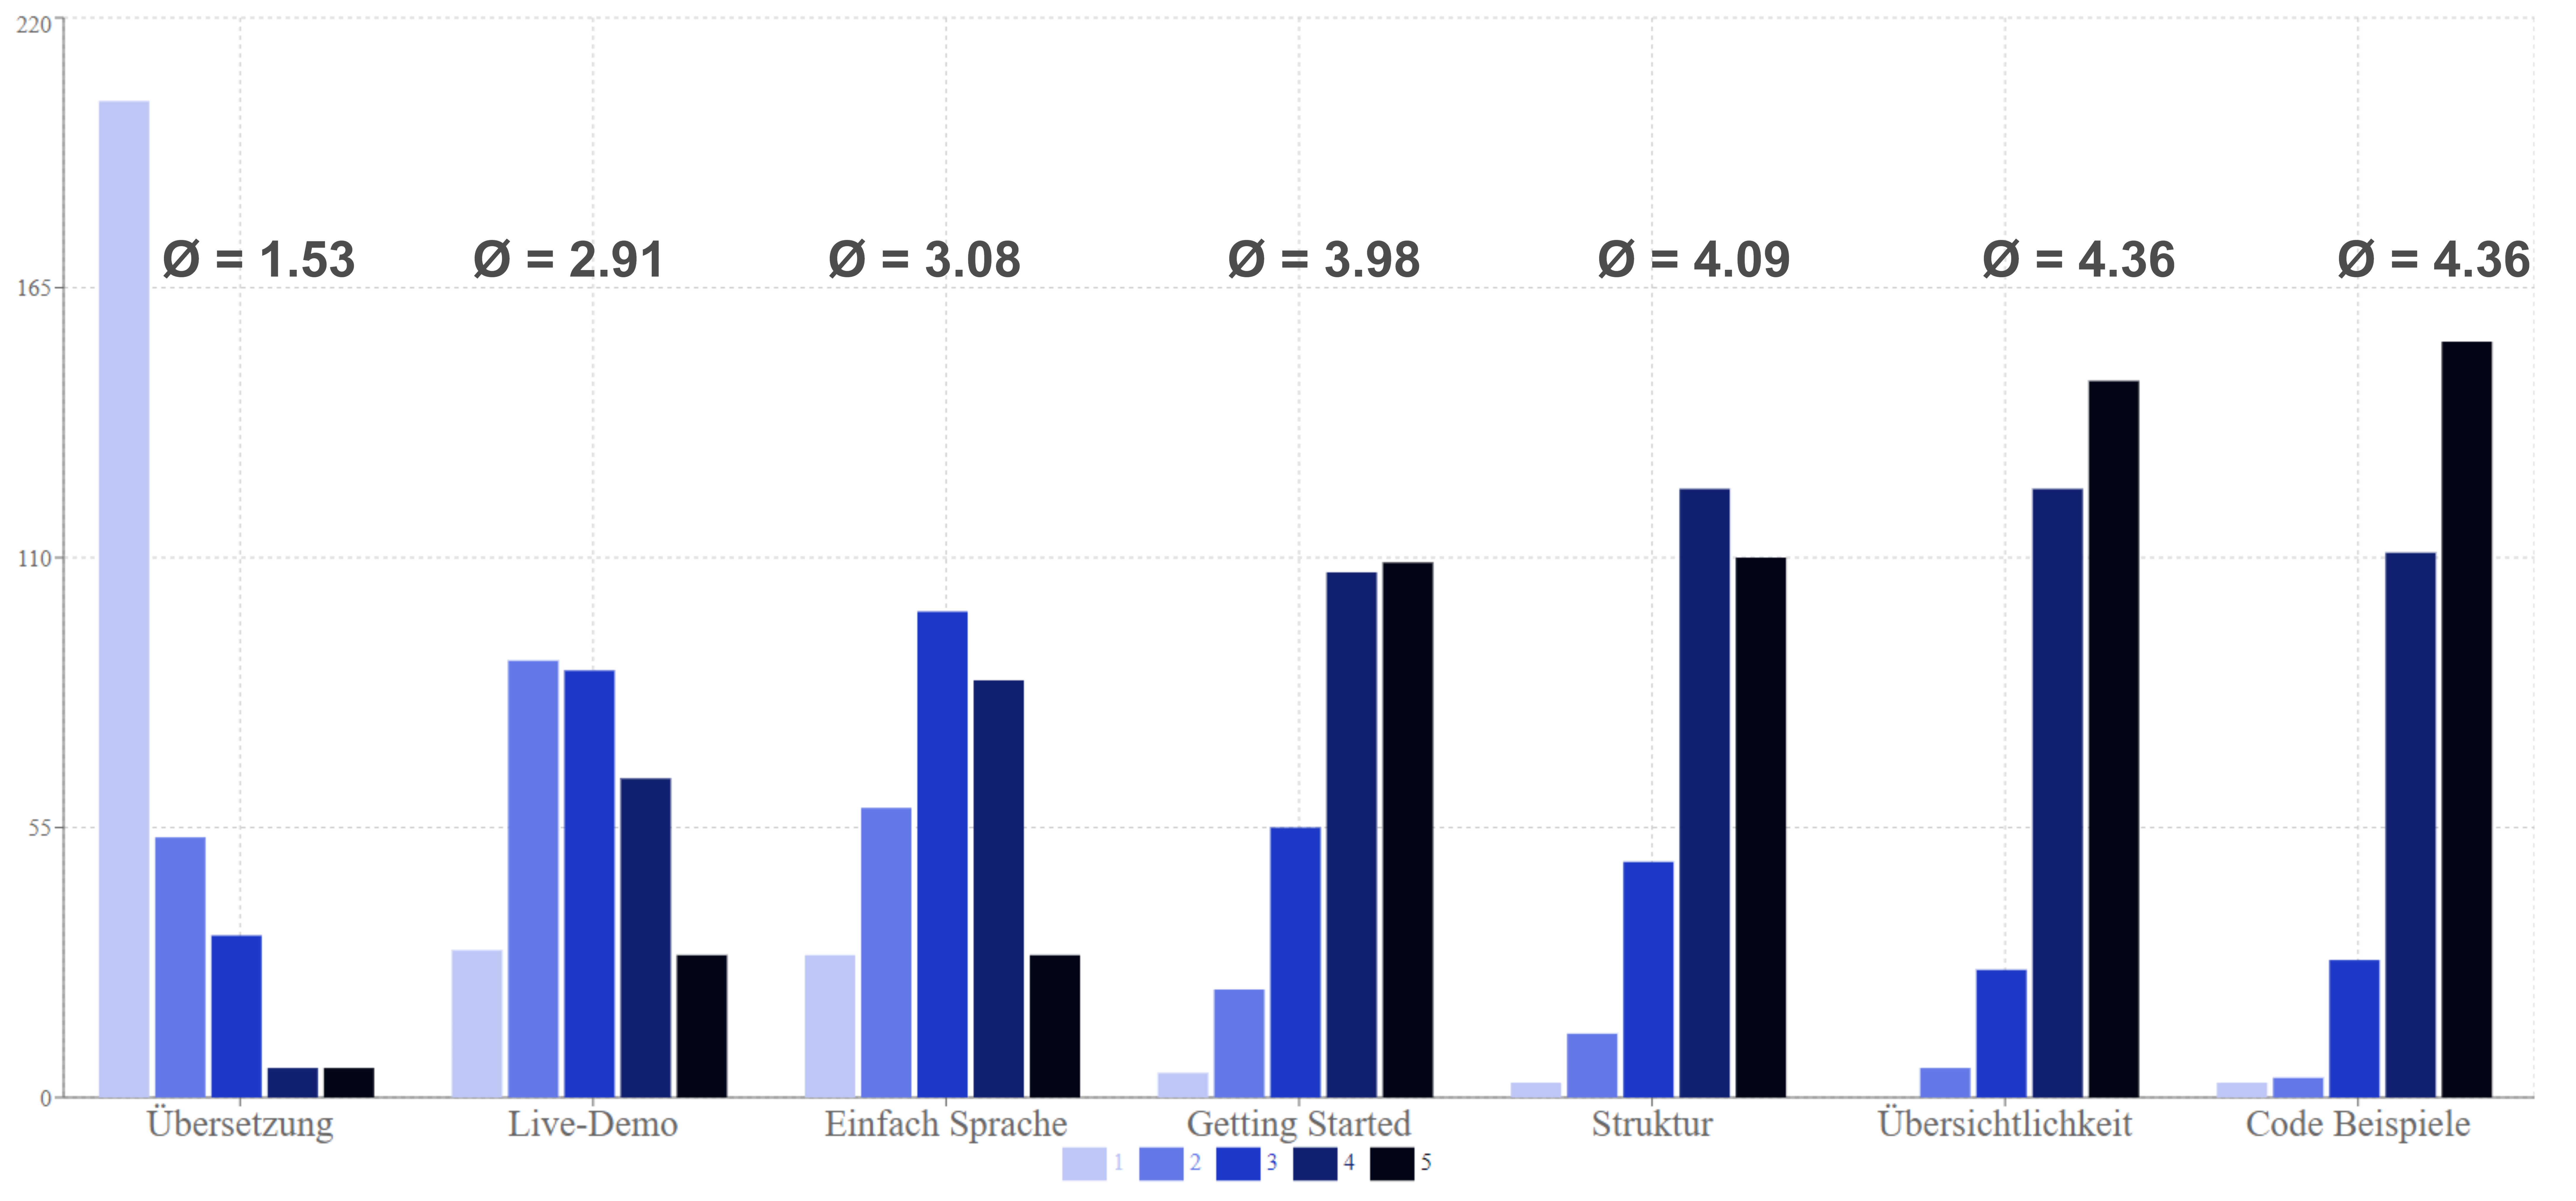
\includegraphics[scale=0.05]{figures/05/GuteDoku_BarChart.png}
    \caption{Antworten: Was zeichnet Gute Dokumentation aus?}
    \label{abb:GuteDoku_BarChart}
\end{figure}

\begin{figure}[h]
    \centering
    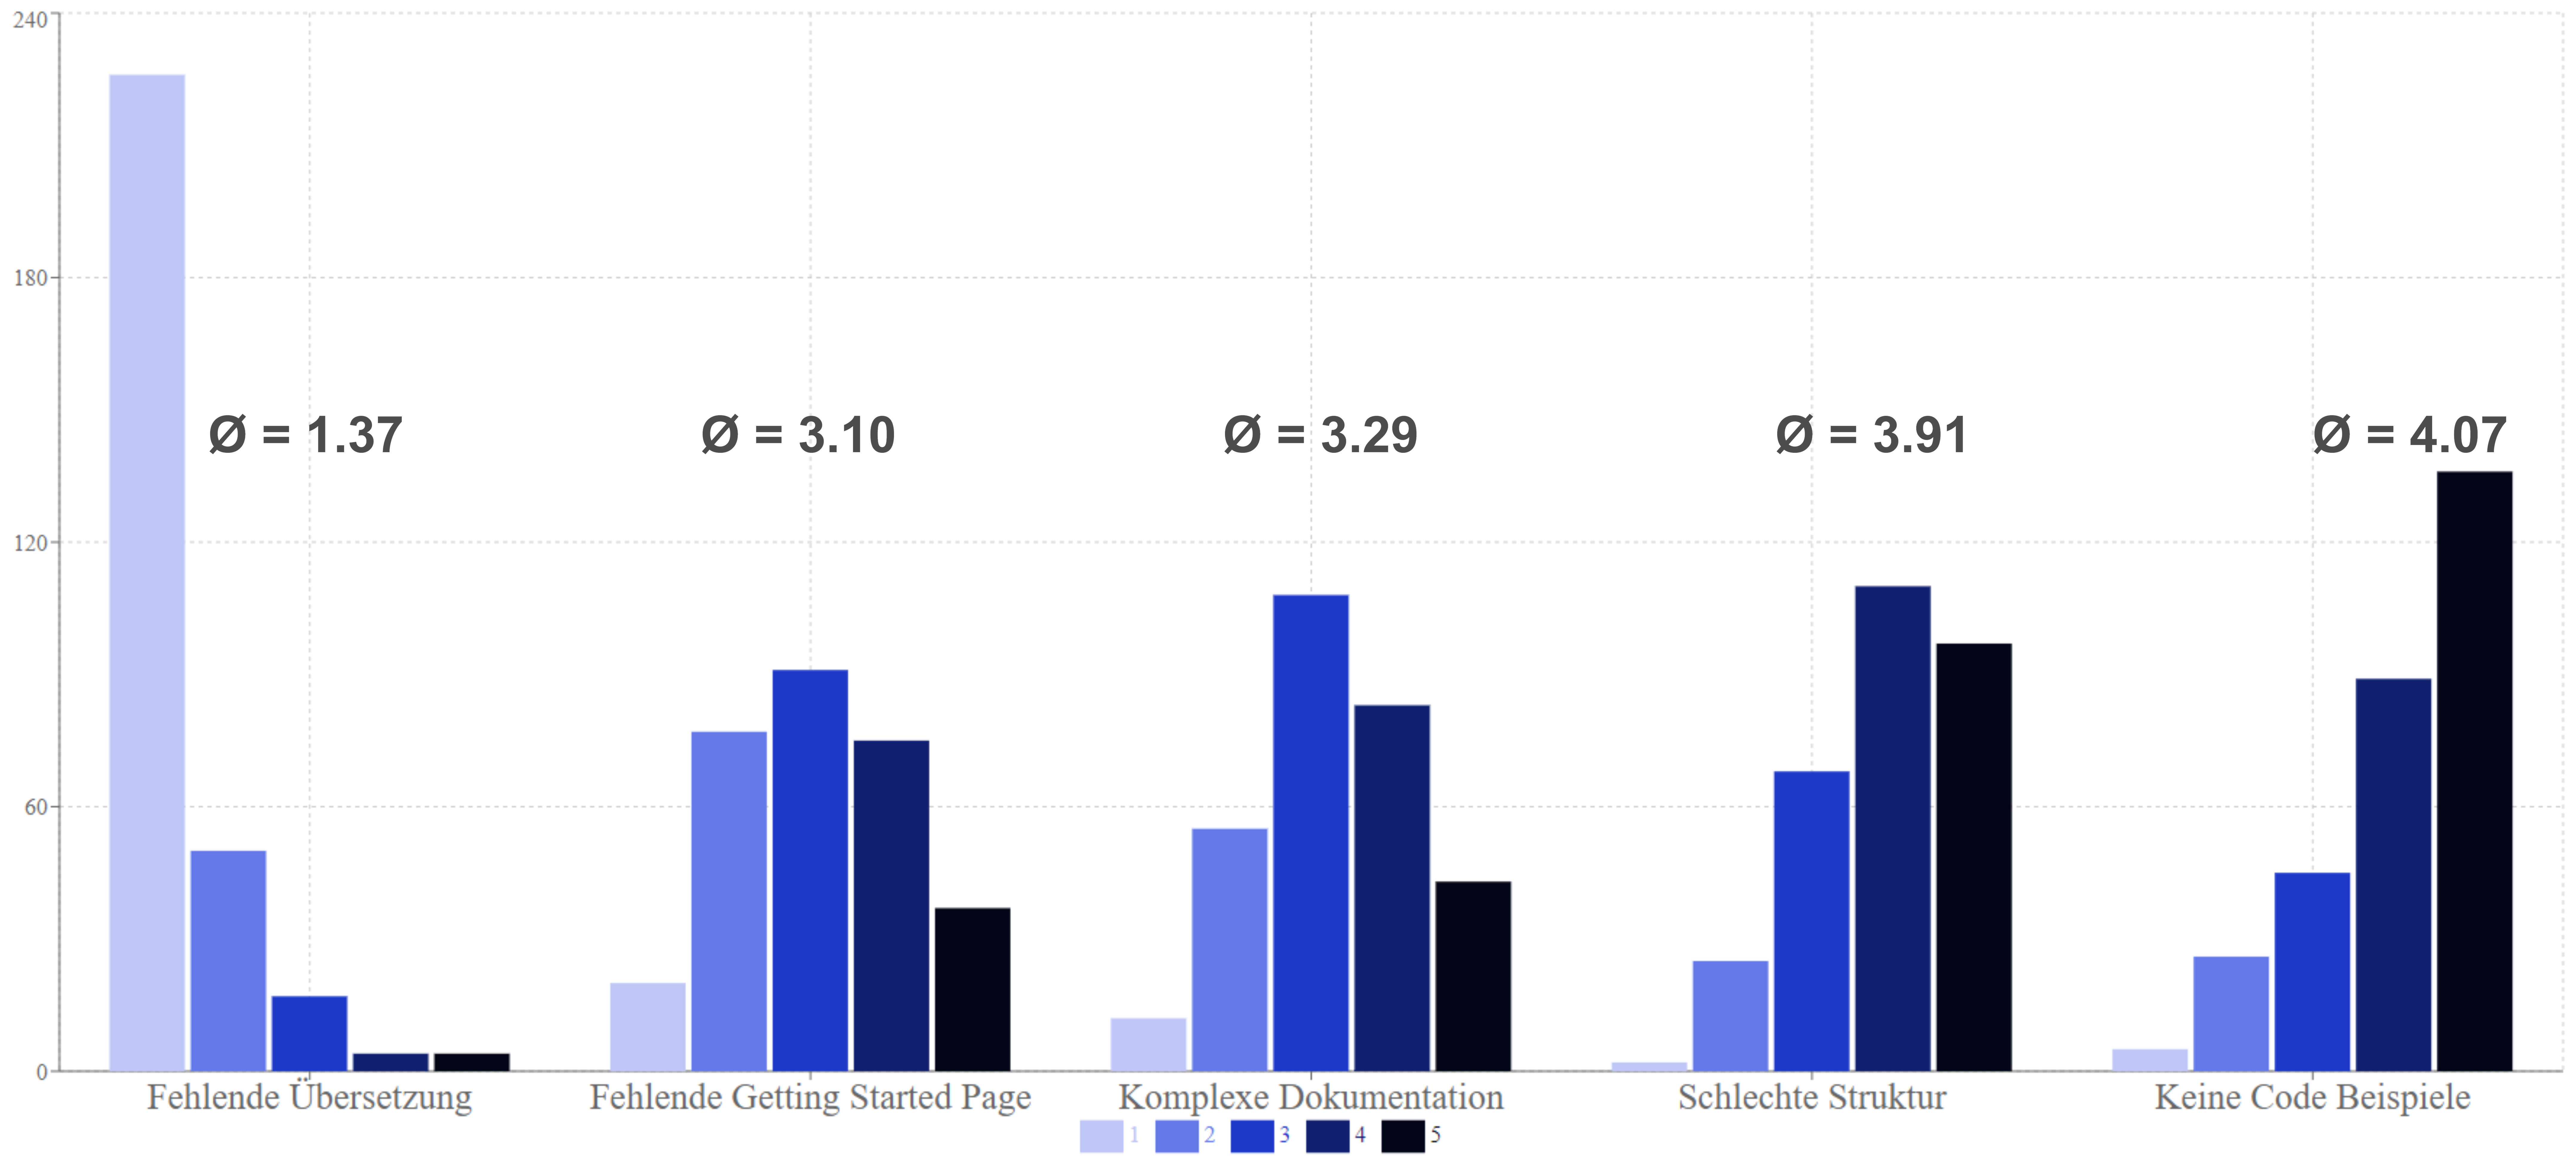
\includegraphics[scale=0.05]{figures/05/SchlechteDoku_BarChart.png}
    \caption{Antworten: Was zeichnet Gute Dokumentation aus?}
    \label{abb:SchlechteDoku_BarChart}
\end{figure}


% Tabelle: Most Used Words
\begin{figure}[tph]
    \todo{Die zwei Tabellen unten werden als \textbf{Abbildung} gekennzeichnet ! Statt Tabellen
    Copy Paste einfach die Tabelle 4.1 Lizenzen der erfassten Projekte}
    \begin{minipage}[t]{0.4\textwidth}\vspace{0pt}%
        \subcaptionbox{\label{tab:gute_doku_freitext}Freitext: Gute Dokumentation}{
            \begin{tabular}{lc}
                \firsthline
                Aktualität          & 28 \\ \hline
                Vollständigkeit     & 21 \\ \hline
                Gute UX             & 14 \\ \hline
                Versionierung       & 10 \\ \hline
                Changelog vorhanden & 6  \\ \hline
                Gute Code Beispiele & 5  \\ \hline
            \end{tabular}% 
        }
    \end{minipage}
    %
    \hfill
    %
    \begin{minipage}[t]{0.5\textwidth}\vspace{0pt}%
        \subcaptionbox{\label{tab:schlechte_doku_freitext}Freitext: Schlechte Dokumentation}{
            \begin{tabular}{lc}
                \firsthline
                Veraltet                           & 25 \\ \hline
                Unvollständig                      & 15 \\ \hline
                Schlechte UX                       & 11 \\ \hline
                Fehlerhaft                         & 7  \\ \hline
                Keine Doku vorhanden               & 6  \\ \hline
                Code Beispiele Funktionieren nicht & 5  \\ \hline
            \end{tabular}% 

        }
    \end{minipage}
    \captionabove{\label{tab:freitext_felder_ergebnisse}Häufigste Erwähnungen beim Freitext}
\end{figure}
